%\documentclass[12pt]{article}
%\usepackage[a4paper, margin=1in]{geometry} 
%\usepackage{graphicx} 
%\usepackage{hyperref}
%\usepackage{float}
%\usepackage{multicol}
%\usepackage{multirow}
%\usepackage{amsmath}
%\usepackage[ruled]{algorithm2e}
%\usepackage[font=small, labelfont=bf]{caption}
%
%\begin{document}

%
% Maximum parsimony
%
\subsection{Maximum parsimony}
Maximum parsimony is a character-based method to reconstruct a phylogenetic tree. 

%
%  Definition of parsimony
%
\subsubsection*{Definition of parsimony}
\begin{figure}[H]
  \centering
      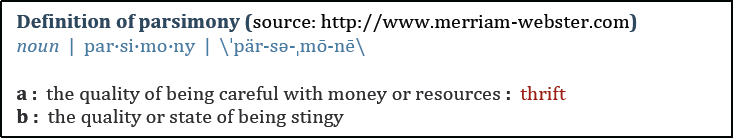
\includegraphics[width=0.7 \textwidth]{fig09/parsimony.png}
\end{figure}

%
%  Tree search method of maximum parsimony 
%
\subsubsection*{Tree search method of maximum parsimony}
The maximum parsimony method uses a tree search to find the tree with the minimum number of mutations. \\

\begin{algorithm}[H]    
  \BlankLine
  Construct an MSA;
  \BlankLine
    
  \ForEach{column $c$ $\in$ MSA}{
    \ForEach{tree $t$ $\in$ all possible topologically different trees}{
      Count the number of union operations in $c$ for tree $t$;
    }
    Add one point to the tree with the minimum union operations;
  }
  
  \BlankLine
  Report the tree with the maximum point;
   \BlankLine
    
  \SetAlgoRefName{\thesection.1}
  \caption{Maximum parsimoney with the minimum union operations}

\end{algorithm}

%
%  Count the number of union operations
%
\subsubsection*{Count the number of union operations}
Either intersection or union operation is performed for each internal node.

\begin{itemize}
\item $s_i=s_j \cap s_k$ \quad If there is at least one element in $s_j$ and $s_k$
\item $s_i=s_j \cup s_k$ \quad Otherwise
\end{itemize}

%
% Example of counting the number of union operations
%
\subsubsection*{Example of counting the number of union operations}
Count the number of union operations for the first and the second columns.

\begin{figure}[H]
  \centering
      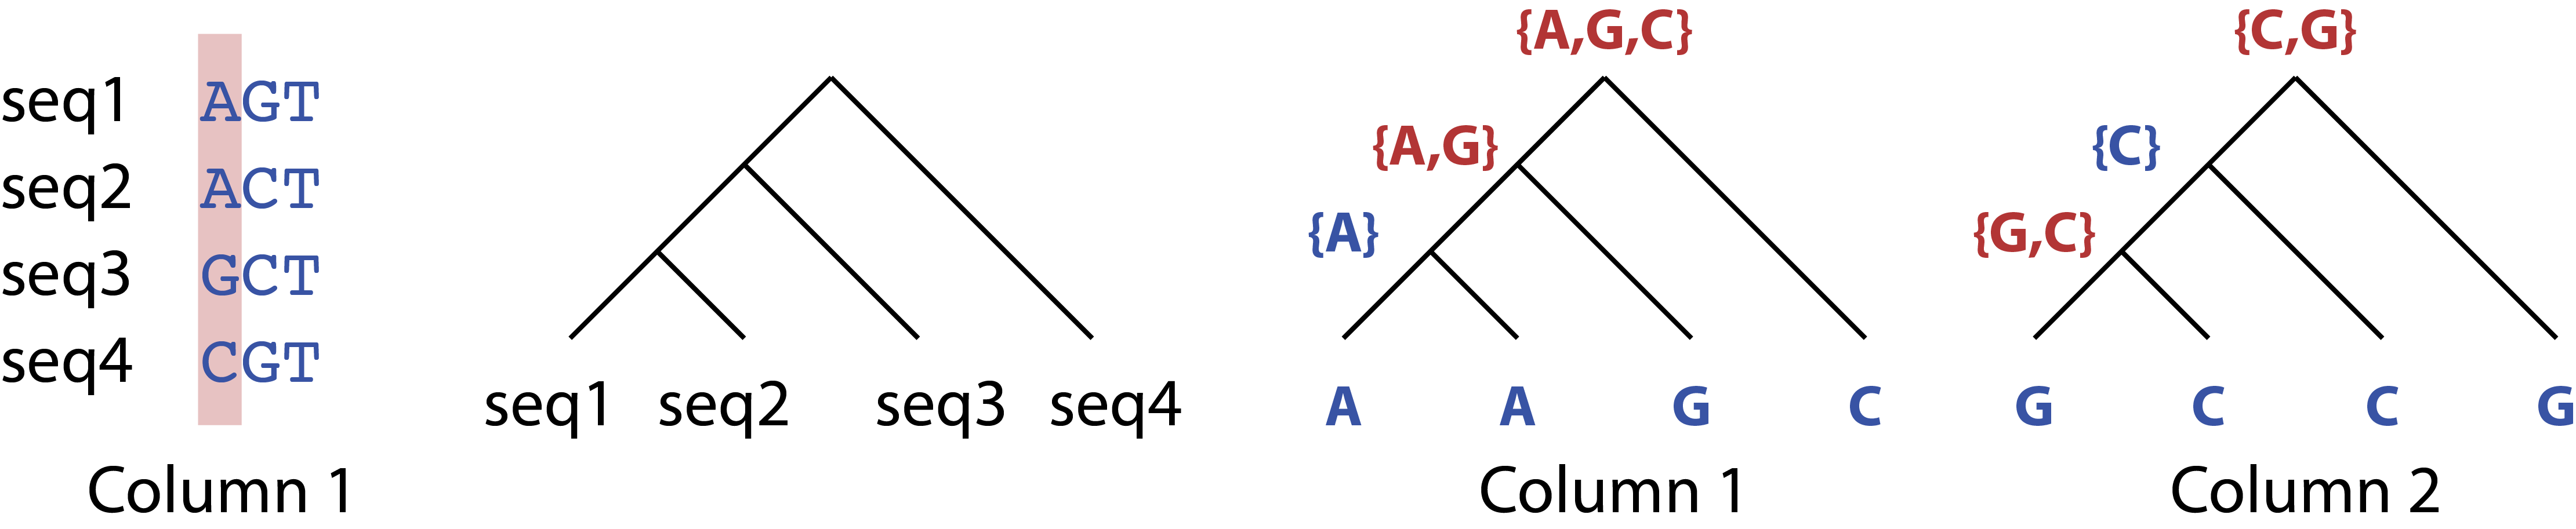
\includegraphics[width=0.8 \textwidth]{fig09/union_operations.png}
\end{figure}

\noindent
\textbf{Colomn 1}
\begin{itemize}
\item $A \cap A \rightarrow \{A\}$ 
\item $\{A\} \cup G \rightarrow \{A, G\}$ 
\item $\{A, G\} \cup C \rightarrow \{A, G, C\}$
\end{itemize}

\# of union opereations: 2

\bigskip 

\noindent
\textbf{Colomn 2}
\begin{itemize}
\item $G \cup C \rightarrow \{G, C\}$ 
\item $\{G, C\} \cap C \rightarrow \{C\}$ 
\item $\{C\} \cup G \rightarrow \{C, G\}$
\end{itemize}

\# of union opereations: 2

%
% Exercise \thesection.3
%
\subsubsection*{Exercise \thesection.3}
\begin{enumerate}
\item What is the number of union operations for the third column?
\begin{figure}[H]
  \centering
      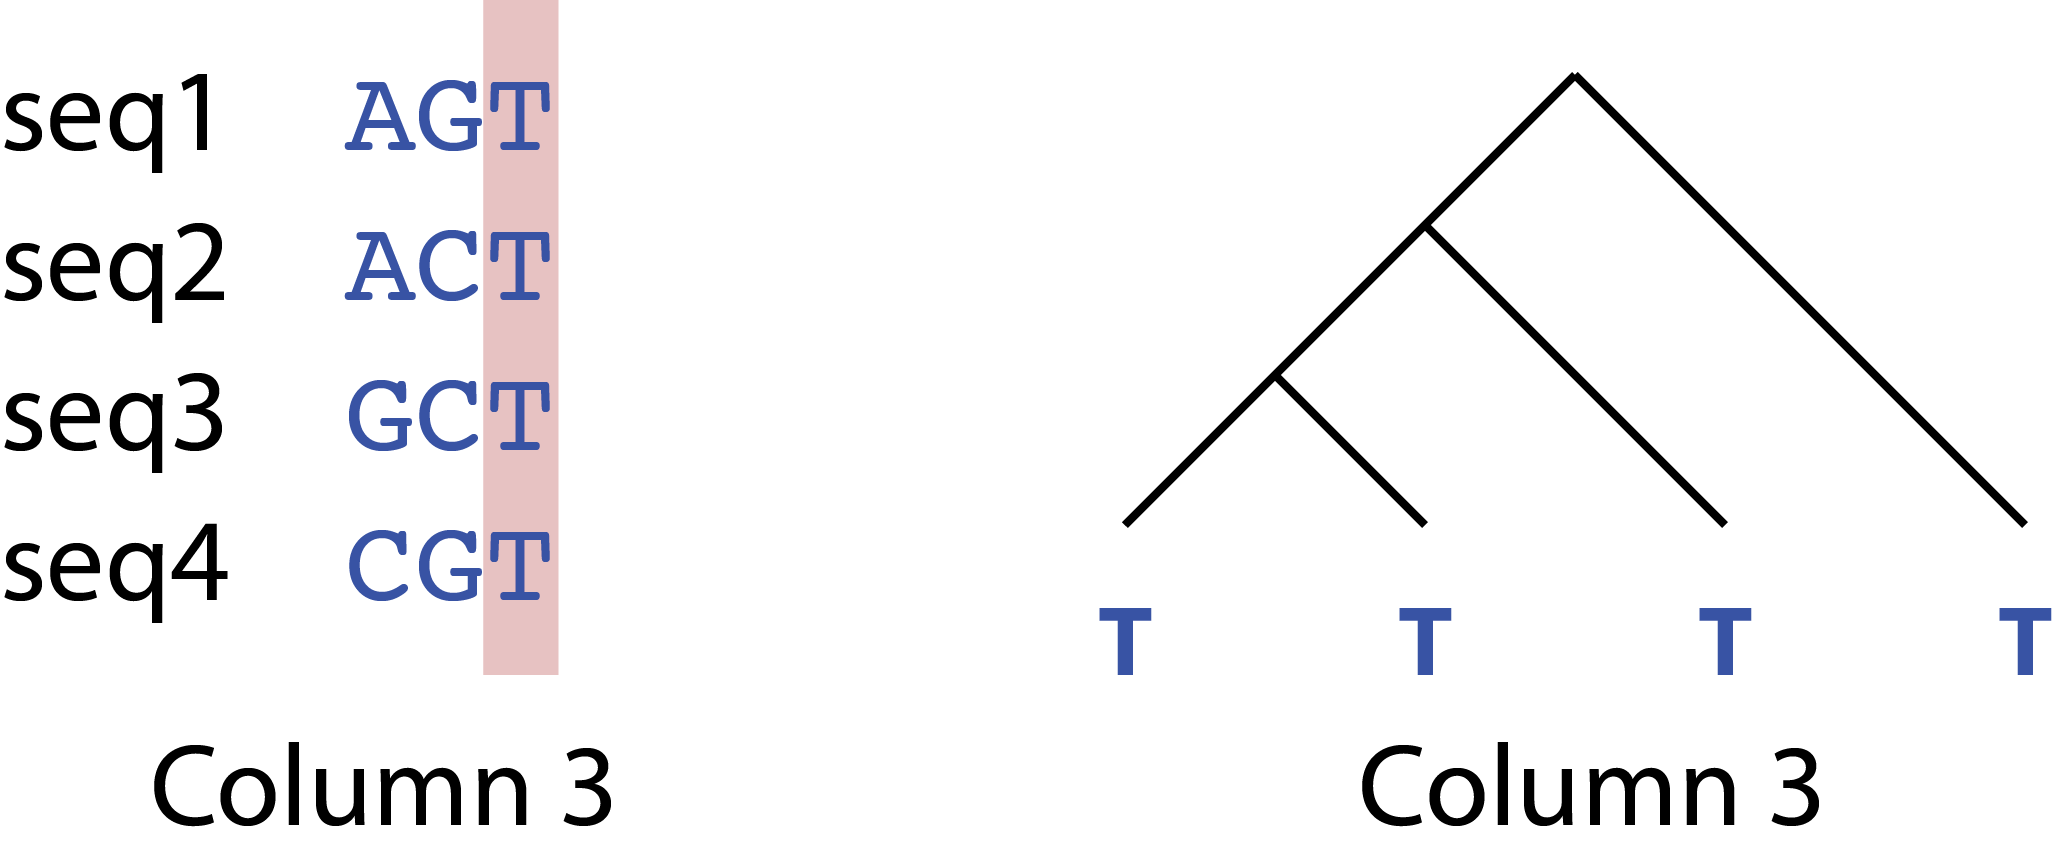
\includegraphics[width=0.4 \textwidth]{fig09/mp_exercise_1.png}
\end{figure}

\item What is the number of union operations for each column?
\begin{figure}[H]
  \centering
      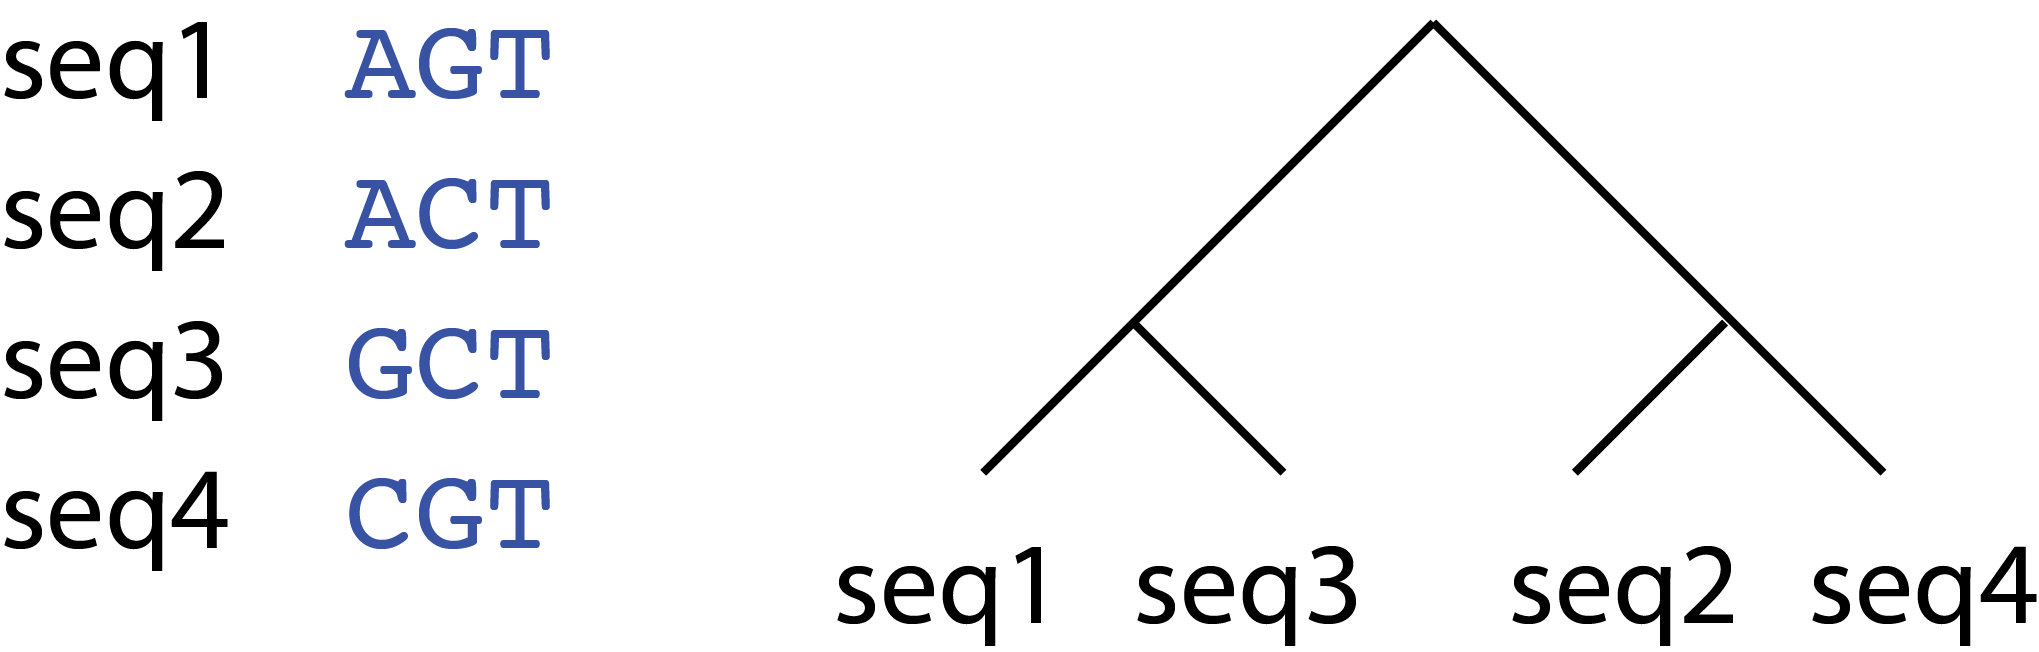
\includegraphics[width=0.4 \textwidth]{fig09/mp_exercise_2.png}
\end{figure}

\begin{itemize}
\item Column 1:
\item Column 2:
\item Column 3:
\end{itemize}

\end{enumerate}

\bigskip 

%\end{document}
